\RequirePackage{amsthm} %https://tex.stackexchange.com/questions/687324/unknown-theoremstyle-warning-with-springer-nature-template
\documentclass[sn-mathphys-num,iicol]{sn-jnl}

%\usepackage{sn-jnl.sty}
\usepackage{graphicx}%
\usepackage{multirow}%
\usepackage{amsmath,amssymb,amsfonts}%
\usepackage{amsthm}%
\usepackage{physics}
\usepackage{siunitx}
\usepackage{mathrsfs}%
\usepackage[title]{appendix}%
\usepackage{xcolor}%
\usepackage{textcomp}%
\usepackage{manyfoot}%
\usepackage{booktabs}%
\usepackage{algorithm}%
\usepackage{algorithmicx}%
\usepackage{algpseudocode}%
\usepackage{listings}%
\usepackage{newtxmath}%
\usepackage[tiny]{titlesec}%
\usepackage[ngerman]{babel}
\usepackage{booktabs}

\theoremstyle{thmstyleone}
\newtheorem{theorem}{Theorem}
\newtheorem{proposition}[theorem]{Proposition}

\theoremstyle{thmstyletwo}
\newtheorem{remark}{Remark}

\theoremstyle{thmstylethree}
\newtheorem{definition}{Definition}

\raggedbottom

\newcommand{\td}{\text{d}}

\titleformat{\subsection}{}{\thesubsection}{1em}{\itshape}
\titleformat{\subsubsection}{}{\thesubsubsection}{1em}{\itshape}

\begin{document}

\title[]{Praktikum 4 -- Versuch 422: Rastertunnelmikroskop}
\author*[1]{\fnm{Jonas} \sur{Wortmann}}\email{s02jwort@uni-bonn.de}
\author*[1]{\fnm{Angelo} \sur{Brade}}\email{s72abrad@uni-bonn.de}
\affil*[1]{Rheinische Friedrich--Wilhelms--Universität, Bonn}

\maketitle

\section{Einführung}

% TODO: Grobe aufteilung. Kann immer geändert werden. Ist jetzt nicht so festgelegt. Nur als Orientierung.
\section{Spitzen}
\section{Gold Probe}
\begin{figure}[t]
        \centering
        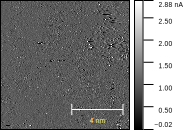
\includegraphics[width=.5\textwidth]{../data/Gold_10nm_current.png}
        \caption{Gold: Strom Karte bei const. current Modus (Setpoint=\SI{1}{\nano A}, P-Gain=\SI{1000}{}, I-Gain=\SI{2000}{} und Tip voltage=\SI{1}{V})} \label{fig:g10nmc}
\end{figure}
\begin{figure}[t]
        \centering
        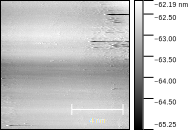
\includegraphics[width=.5\textwidth]{../data/Gold_10nm_z.png}
        \caption{Gold: Höhen Karte bei const. current Modus (Setpoint=\SI{1}{\nano A}, P-Gain=\SI{1000}{}, I-Gain=\SI{2000}{} und Tip voltage=\SI{1}{V})} \label{fig:g10nmz}
\end{figure}
\begin{figure}[t]
        \centering
        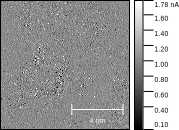
\includegraphics[width=.5\textwidth]{../data/Gold_10nm_50mV_current.png}
        \caption{Gold: Strom Karte bei const. current Modus (Setpoint=\SI{1}{\nano A}, P-Gain=\SI{1000}{}, I-Gain=\SI{2000}{} und Tip voltage=\SI{50}{\milli V})} \label{fig:g10nm50mVc}
\end{figure}
\begin{figure}[t]
        \centering
        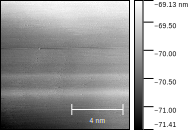
\includegraphics[width=.5\textwidth]{../data/Gold_10nm_50mV_z.png}
        \caption{Gold: Höhen Karte bei const. current Modus (Setpoint=\SI{1}{\nano A}, P-Gain=\SI{1000}{}, I-Gain=\SI{2000}{} und Tip voltage=\SI{50}{\milli V})} \label{fig:g10nm50mVz}
\end{figure}
\begin{figure}[t]
        \centering
        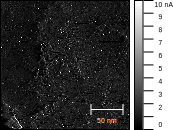
\includegraphics[width=.5\textwidth]{../data/Gold_200nm_current.png}
        \caption{Gold: Strom Karte bei const. current Modus (Setpoint=\SI{1}{\nano A}, P-Gain=\SI{1000}{}, I-Gain=\SI{2000}{} und Tip voltage=\SI{1}{V})} \label{fig:g200nmc}
\end{figure}
\begin{figure}[t]
        \centering
        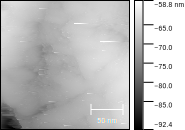
\includegraphics[width=.5\textwidth]{../data/Gold_200nm_z.png}
        \caption{Gold: Höhen Karte bei const. current Modus (Setpoint=\SI{1}{\nano A}, P-Gain=\SI{1000}{}, I-Gain=\SI{2000}{} und Tip voltage=\SI{1}{V})} \label{fig:g200nmz}
\end{figure}
\begin{figure}[t]
        \centering
        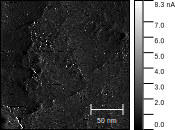
\includegraphics[width=.5\textwidth]{../data/Gold_200nm_50mV_current.png}
        \caption{Gold: Strom Karte bei const. current Modus (Setpoint=\SI{1}{\nano A}, P-Gain=\SI{1000}{}, I-Gain=\SI{2000}{} und Tip voltage=\SI{50}{\milli V})} \label{fig:g200nm50mVc}
\end{figure}
\begin{figure}[t]
        \centering
        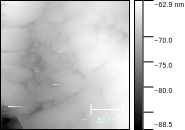
\includegraphics[width=.5\textwidth]{../data/Gold_200nm_50mV_z.png}
        \caption{Gold: Höhen Karte bei const. current Modus (Setpoint=\SI{1}{\nano A}, P-Gain=\SI{1000}{}, I-Gain=\SI{2000}{} und Tip voltage=\SI{50}{\milli V})} \label{fig:g200nm50mVz}
\end{figure}
\begin{figure}[t]
        \centering
        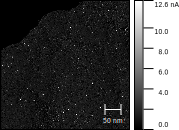
\includegraphics[width=.5\textwidth]{../data/Gold_400nm_current.png}
        \caption{Gold: Strom Karte bei const. current Modus (Setpoint=\SI{1}{\nano A}, P-Gain=\SI{1000}{}, I-Gain=\SI{2000}{} und Tip voltage=\SI{1}{V})} \label{fig:g400nmc}
\end{figure}
\begin{figure}[t]
        \centering
        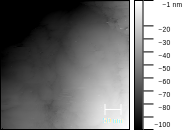
\includegraphics[width=.5\textwidth]{../data/Gold_400nm_z.png}
        \caption{Gold: Höhen Karte bei const. current Modus (Setpoint=\SI{1}{\nano A}, P-Gain=\SI{1000}{}, I-Gain=\SI{2000}{} und Tip voltage=\SI{1}{V})} \label{fig:g400nmz}
\end{figure}
\section{Graphit Probe}
% TODO: Beachte, dass die beiden pngs hier mit 1V benannte sind, aber eigentlich 50mV Tip voltage hatten
\begin{figure}[t]
        \centering
        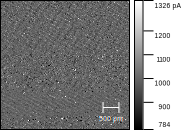
\includegraphics[width=.5\textwidth]{../data/Graphit_4nm_1V_current.png}
        \caption{Gold: Strom Karte bei const. current Modus (Setpoint=\SI{1}{\nano A}, P-Gain=\SI{1000}{}, I-Gain=\SI{2000}{} und Tip voltage=\SI{50}{\nano V})} \label{fig:gr4nm50mVc}
\end{figure}
\begin{figure}[t]
        \centering
        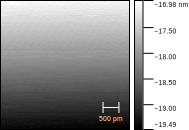
\includegraphics[width=.5\textwidth]{../data/Graphit_4nm_1V_z.png}
        \caption{Gold: Höhen Karte bei const. current Modus (Setpoint=\SI{1}{\nano A}, P-Gain=\SI{1000}{}, I-Gain=\SI{2000}{} und Tip voltage=\SI{50}{\nano V})} \label{fig:gr4nm50mVz}
\end{figure}


\bibliography{refs}

\end{document}
